\documentclass[12pt]{article}
\usepackage[utf8]{inputenc}
\usepackage{graphicx}
\usepackage[a4paper,width=150mm,top=25mm,bottom=25mm]{geometry}

\title{

\\
{COS 301 SRS}
}



\author{Ctrl Alt Defeat}


\begin{document}

\begin{titlepage}
    \centering



    \vspace{2cm}
    \hrulefill\\
    \vspace{1cm}
    {\Huge\bfseries SRS Documentation v3.0}

    \vspace{1cm}

    {\Large Software Requirements Specification Document for\\Domain Pulse}\\
    \vspace{1cm}
    \hrulefill\\

    \vfill

    {\large Ctrl Alt Defeat}

    \vspace{1cm}

    {\large 2023/07/31}\\
    %    \vspace{1cm}
    %    \vspace{1cm}
    %    
\includegraphics[width=10cm]{../../Images/dpLogo.png}
    %    \vspace{1cm}\\
    %    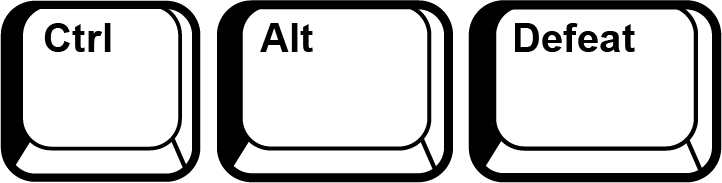
\includegraphics[width=6cm]{../../Images/cadLogo.png}

\end{titlepage}




\tableofcontents

\newpage











\section{Introduction}

\subsection{Overview}
Introducing Domain Pulse, the ultimate sentiment analysis platform. With Domain Pulse, you can easily gauge the sentiment surrounding any domain. Whether it's a business, franchise, a product, an event, or more. Domain Pulse gathers and analyzes sentiment data from various sources, ranging from social media to review platforms, with the support for providing your own data either via a live review process or a CSV.\\
\\Domain Pulse presents the results in a visually stunning and easy-to-understand format. Our wide range of visualizations brings statistics to life, making it a breeze to grasp the online presence and sentiment for any domain. Take control of understanding public opinion like never before with Domain Pulse.
\subsection{Objectives}

The objectives of the Domain Pulse project are to develop a comprehensive web application that enables users to track and analyze data from multiple sources, perform sentiment analysis, and visualize statistics. The application aims to provide a user-centered design approach, ensuring usability, accessibility, and a clear and intuitive interface. The system will be built using a scalable and modifiable architecture, leveraging a combination of powerful architectural patterns to achieve the quality requirements set out in the Architectural Design document and statement of quality requirements.

\newpage













\section{User Characteristics}

Domain Pulse caters to a diverse range of users with varying demographics, ranging from high-school students to more mature age groups. Domain Pulse can be used by people with various educational backgrounds and professional roles. These may include business professionals, social media managers, researchers, and PR professionals - however other users may find value in using Domain Pulse by simply satisfying personal interests and exploration.\\\\
Despite the diverse background of our users, they are all unified by their personal and professional interests, with a keen interest in sentiment analysis, online presence monitoring, and understanding public perception. They value data-driven decision-making and insights to support their decision-making processes. Additionally, they have a strong interest in market research, branding, reputation management, and online sentiment analysis. With their analytical and exploratory-oriented mindsets, these users are driven to monitor and/or manage online presence and sentiment, exploring their personal and professional interests with Domain Pulse.\\\\
Regarding the technological proficiency of users, Domain Pulse accommodates individuals at different skill levels. Novice users, who possess basic technological skills, may require more guidance, while intermediate users have moderate experience and comfort using technology. Expert users, on the other hand, are technologically proficient and adapt quickly to new systems.\\\\
In terms of prior knowledge and experience, users may have different levels of expertise in sentiment analysis and online presence monitoring, as well as varying degrees of familiarity with similar tools or platforms.

\newpage
















\section{User Stories}

\subsection{First Iteration}
\begin{table}[htbp]
  \caption{User Story: Add a domain}
  \begin{tabular}{|p{0.45\textwidth}|p{0.45\textwidth}|}
    \hline
    \textbf{User Story}          & As a user/business manager, I want to add a domain (business, product, etc...) to my list of domains, so that I can view and track customers' sentiment of it. \\
    \hline
    \textbf{Acceptance Criteria} &
    Given that I provided the name of the domain I wish to track,                                                                                                                                 \\
                                 & When I click the 'add domain' button,                                                                                                                          \\
                                 & Then the domain is added to my list.                                                                                                                           \\
    \hline
  \end{tabular}
\end{table}

\begin{table}[htbp]
  \caption{User Story: Remove a domain}
  \begin{tabular}{|p{0.45\textwidth}|p{0.45\textwidth}|}
    \hline
    \textbf{User Story}          & As a user/business manager, I want to remove a domain (business, product, etc...) from my list of domains, so that I can remove unimportant or unneeded domains. \\
    \hline
    \textbf{Acceptance Criteria} &
    Given that I have selected the domain I wish to remove,                                                                                                                                         \\
                                 & When I click the 'remove domain' button,                                                                                                                         \\
                                 & Then the domain is removed from my list.                                                                                                                         \\
    \hline
  \end{tabular}
\end{table}

\begin{table}[htbp]
  \caption{User Story: Selecting a website theme}
  \begin{tabular}{|p{0.45\textwidth}|p{0.45\textwidth}|}
    \hline
    \textbf{User Story}          & As a user, I want to change the theme to light or dark mode for my personal preference, so that I can more enjoy my use of the web-app. \\
    \hline
    \textbf{Acceptance Criteria} &
    Given that I am within the web-app,                                                                                                                                    \\
                                 & When I click the 'Change Theme' button,                                                                                                 \\
                                 & Then the theme of the page is changed.                                                                                                  \\
    \hline
  \end{tabular}
\end{table}
\begin{table}[htbp]
  \caption{User Story: Log out of an account}
  \begin{tabular}{|p{0.45\textwidth}|p{0.45\textwidth}|}
    \hline
    \textbf{User Story}          & As a user, I want to log out of my account, so that I can log in on another or have more security of others not viewing my domains. \\
    \hline
    \textbf{Acceptance Criteria} &
    Given that I am currently signed into an account,                                                                                                                  \\
                                 & When I click the 'Sign Out' button,                                                                                                 \\
                                 & Then I am signed out of my account and placed on the login page.                                                                    \\
    \hline
  \end{tabular}
\end{table}
\begin{table}[htbp]
  \caption{User Story: Add a source}
  \begin{tabular}{|p{0.45\textwidth}|p{0.45\textwidth}|}
    \hline
    \textbf{User Story}          & As a user/business manager, I want to add a source (Youtube, Google Reviews, etc...) for sentiment data to my list of sources, so that I can view and track customers' sentiment on said source. \\
    \hline
    \textbf{Acceptance Criteria} &
    Given that I provided the name/link to the source I wish to use,                                                                                                                                                           \\
                                 & When I click the 'add source' button and select the appropriate source type (providing the appropriate parameter data),                                                                                                                                                       \\
                                 & Then the source is added to my list of sources.                                                                                                                                             \\
    \hline
  \end{tabular}
\end{table}

\begin{table}[htbp]
  \caption{User Story: Select a domain}
  \begin{tabular}{|p{0.45\textwidth}|p{0.45\textwidth}|}
    \hline
    \textbf{User Story}          & As a user/business manager, I want to select a domain (business, product, etc...) from my list of domains, so that I can view and track customers' sentiment regarding it and other pieces of meta-data regarding the sentiment. \\
    \hline
    \textbf{Acceptance Criteria} &
    Given that I have the domain I wish to view in my list of domains,                                                                                                                                                                                              \\
                                 & When I click the domain's name in the list,                                                                                                                                                                                      \\
                                 & Then the sources from where I pull data from are listed and the overall sentiment is displayed.                                                                                                                                  \\
    \hline
  \end{tabular}
\end{table}

\begin{table}[htbp]
  \caption{User Story: Register an account}
  \begin{tabular}{|p{0.45\textwidth}|p{0.45\textwidth}|}
    \hline
    \textbf{User Story}          & As a user, I want to create an account, so that I help my domains perform better by understanding if customers are satisfied by tracking customer sentiment. \\
    \hline
    \textbf{Acceptance Criteria} &
    Given that I have provided my email and password on the 'register' page,                                                                                                                    \\
                                 & When I click the 'Register' button,                                                                                                                          \\
                                 & Then my account is created and I am logged in.                                                                                                               \\
    \hline
  \end{tabular}
\end{table}

\begin{table}[htbp]
  \caption{User Story: Update Password}
  \begin{tabular}{|p{0.45\textwidth}|p{0.45\textwidth}|}
    \hline
    \textbf{User Story}          & As a user, I want to update my password, so that I can ensure the safety of my account or change it to one I shall remember. \\
    \hline
    \textbf{Acceptance Criteria} &
    Given that I am logged into an account,                                                                                                                     \\
                                 & When I click the 'Update Password' button,                                                                                   \\
                                 & Then I am prompted to verify by email if I want to update my password and enter my new password.                             \\
    \hline
  \end{tabular}
\end{table}
\begin{table}[htbp]
  \caption{User Story: Remove a source}
  \begin{tabular}{|p{0.45\textwidth}|p{0.45\textwidth}|}
    \hline
    \textbf{User Story}          & As a user/business manager, I want to remove a source (Twitter, Instagram, etc…) for sentiment data from my list of sources, so as to remove an unhelpful or unwanted source of data. \\
    \hline
    \textbf{Acceptance Criteria} &
    Given that I have selected the source I wish to remove,                                                                                                                                                              \\
                                 & When I click the 'remove source' button,                                                                                                                                              \\
                                 & Then the source is removed from my list of sources.                                                                                                                                   \\
    \hline
  \end{tabular}
\end{table}

\begin{table}[htbp]
  \caption{User Story: Select a domain}
  \begin{tabular}{|p{0.45\textwidth}|p{0.45\textwidth}|}
    \hline
    \textbf{User Story}          & As a user/business manager, I want to select a domain (business, product, etc...) from my list of domains, so that I can view and track customers' sentiment regarding it. \\
    \hline
    \textbf{Acceptance Criteria} &
    Given that I have the domain I wish to view in my list of domains,                                                                                                                                        \\
                                 & When I click the domain's name in the list,                                                                                                                                \\
                                 & Then display the overall sentiment and list of sources selected for that domain.                                                                                           \\
    \hline
  \end{tabular}
\end{table}

\begin{table}[htbp]
  \caption{User Story: Log into an account}
  \begin{tabular}{|p{0.45\textwidth}|p{0.45\textwidth}|}
    \hline
    \textbf{User Story}          & As a user, I want to log into my account, so that I help my domains perform better by understanding if customers are satisfied by tracking customer sentiment. \\
    \hline
    \textbf{Acceptance Criteria} &
    Given that I am not currently signed into an account, on the 'log-in' page and have my account details entered,                                                                               \\
                                 & When I click the 'Log In' button,                                                                                                                              \\
                                 & Then I am logged into my account that stores my previously created domains and sources.                                                                        \\
    \hline
  \end{tabular}
\end{table}

% \begin{table}[htbp]
%   \caption{User Story: Forgot Password}
%   \begin{tabular}{|p{0.45\textwidth}|p{0.45\textwidth}|}
%     \hline
%     \textbf{User Story}          & As a user, I want to update my password, so that I can change it to one I shall remember and access my account. \\
%     \hline
%     \textbf{Acceptance Criteria} &
%     Given that I am on the log-in screen,                                                                                                          \\
%                                  & When I click the 'Forgot Password' button,                                                                      \\
%                                  & Then I am prompted to verify by email if I want to update my password and enter my new password.                \\
%     \hline
%   \end{tabular}
% \end{table}

\begin{table}[htbp]
  \caption{User Story: Select a source}
  \begin{tabular}{|p{0.45\textwidth}|p{0.45\textwidth}|}
    \hline
    \textbf{User Story}          & As a user/business manager, I want to select a source (Twitter, Facebook, etc...) from my list of sources for a domain, so that I can view and track customers' sentiment regarding my domain within the source. \\
    \hline
    \textbf{Acceptance Criteria} &
    Given that I have selected a domain and have provided sources for said domain,                                                                                                                                                                  \\
                                 & When I click the source in the list,                                                                                                                                                                             \\
                                 & Then the overall sentiment specific to the source is displayed.                                                                                                                                                  \\
    \hline
  \end{tabular}
\end{table}

\begin{table}[htbp]
  \caption{User Story: Select a statistic}
  \begin{tabular}{|p{0.45\textwidth}|p{0.45\textwidth}|}
    \hline
    \textbf{User Story}          & As a user/business manager, I want to select a statistic (sentiment or metadata) from all available statistics, so that I can gain a better insight into how that statistic compares to other statistics and how it affects the overall sentiment. \\
    \hline
    \textbf{Acceptance Criteria} &
    Given that sentiment analysis has been performed,                                                                                                                                                                                                                                 \\
                                 & When I click on a specific statistic,                                                                                                                                                                                                              \\
                                 & Then a visualization of the statistic is displayed.                                                                                                                                                                                                \\
    \hline
  \end{tabular}
\end{table}

\begin{table}[htbp]
  \caption{User Story: View source data}
  \begin{tabular}{|p{0.45\textwidth}|p{0.45\textwidth}|}
    \hline
    \textbf{User Story}          & As a user/business manager, I want to be able to see examples of data that was retrieved from my sources, so that I can confirm that the correct source was specified and correctly retrieved. \\
    \hline
    \textbf{Acceptance Criteria} &
    Given that sentiment analysis has been performed,                                                                                                                                                                             \\
                                 & When I am viewing the source of a domain,                                                                                                                                                      \\
                                 & Then the raw source data is also displayed.                                                                                                                                                    \\
    \hline
  \end{tabular}
\end{table}

\begin{table}[htbp]
  \caption{User Story: View source data sentiments}
  \begin{tabular}{|p{0.45\textwidth}|p{0.45\textwidth}|}
    \hline
    \textbf{User Story}          & As a user/business manager, I want to be able to see what the application predicts people think based on what they have said, so that I can confirm the validity of the application’s predictions and trust the system. \\
    \hline
    \textbf{Acceptance Criteria} &
    Given that sentiment analysis has been performed,                                                                                                                                                                                                      \\
                                 & When I am viewing the examples raw source data of a domain,                                                                                                                                                             \\
                                 & Then the predicted sentiment is displayed along with it.                                                                                                                                                                \\
    \hline
  \end{tabular}
\end{table}
\newpage
% \subsection{Later Iterations}
\begin{table}[htbp]
  \caption{User Story: View Time Series data}
  \begin{tabular}{|p{0.45\textwidth}|p{0.45\textwidth}|}
    \hline
    \textbf{User Story}          & As a user/business manager, I want to view the time series data of a domain's sentiment from customers, so that I can understand when customers most enjoyed or disliked my product. \\
    \hline
    \textbf{Acceptance Criteria} &
    Given that I have selected the domain or source I wish to see time series data on,                                                                                                                                            \\
                                 & When I click the navigate the graph pane,                                                                                                                                               \\
                                 & Then the page displays a graph of customer sentiment of the selected domain or source over a period of time.                                                                                   \\
    \hline
  \end{tabular}
\end{table}


\begin{table}[htbp]
  \caption{User Story: Report generation}
  \begin{tabular}{|p{0.45\textwidth}|p{0.45\textwidth}|}
    \hline
    \textbf{User Story}          & As a user/PR manager, I want to generate a sharable PDF report that neatly summarizes the results of the sentiment analysis, so that I can present the results in a meeting or to an executive more formally. \\
    \hline
    \textbf{Acceptance Criteria} &
    Given that I have selected the domain I wish to generate a report for,                                                                                                                                            \\
                                 & When click the "Generate report" button,                                                                                                                                               \\
                                 & Then a QR code is displayed as well as a URL to view the PDF report.                                                                                   \\
    \hline
  \end{tabular}
\end{table}


\begin{table}[htbp]
  \caption{User Story: Live review}
  \begin{tabular}{|p{0.45\textwidth}|p{0.45\textwidth}|}
    \hline
    \textbf{User Story}          & As a user/PR manager, I want to generate a QR code that enables anyone to make a review about any arbitrary thing, so that I may collect my own sentiment data in real time. \\
    \hline
    \textbf{Acceptance Criteria} &
    Given that I have selected the domain I wish to add a live review data source to,                                                                                                                                            \\
                                 & When click the "Add source" button and select live review,                                                                                                                                               \\
                                 & Then a QR code is displayed which acts as a link to the review form.                                                                                   \\
    \hline
  \end{tabular}
\end{table}

\newpage

\section{Functional Requirements}

 (grouped by subsystems)

\subsection{Authentication}
\begin{enumerate}
  \item Registration
        \begin{enumerate}
          \item Can register using username and password
        \end{enumerate}
  \item Login
        \begin{enumerate}
          \item Can login using username and password
        \end{enumerate}
  \item Log out
        \begin{enumerate}
          \item A user has a means whereby they can log out of their account
        \end{enumerate}
  \item Update password
        \begin{enumerate}
          \item A user may securely change their password
        \end{enumerate}
  \item Remove account
        \begin{enumerate}
          \item A user can delete their account
        \end{enumerate}
\end{enumerate}

\subsection{Domain management}
\begin{enumerate}
  \item A user may create and domains with custom names, the domain acts as a 'folder' for a number of sources of data
  \item A user may add a description for a domain
  \item A user may add an image or select an icon to represent the domain
  \item A user may remove a domain
  \item Within a domain, the following operations can be performed
        \begin{enumerate}
          \item Add a data source (ex: Comments on a specified Youtube video) by selecting a source type and specifying a URL for that source
          \item Remove a data source
          \item The following sources must be available for analysis:
                \begin{enumerate}
                  \item Youtube
                  \item Google reviews
                  \item Tripadvisor
                  \item TrustPilot
                  \item Live review \begin{itemize}
                    \item A user can toggle whether the review is enabled or disabled 
                    \item A user is presented with a QR code that can be shared - linking to a review form
                  \end{itemize}
                  \item CSV upload
                \end{enumerate}
          \item Refresh the data for the whole domain or a singular source
          \item Edit a source's name
        \end{enumerate}
  \item A user can delete domains (which should delete the sources within the domain too)
\end{enumerate}


\subsection{Sentiment Analysis}
\begin{enumerate}
  \item Sentiment analysis can be performed within any of the following groupings
        \begin{enumerate}
          \item For the domain as a whole (this includes all data across all specified sources)
          \item Per data source (this considers all the data retrieved from one specific source)
        \end{enumerate}
  \item The results of sentiment analysis on a grouping are returned as follows
        \begin{enumerate}
          \item The ratios of positive, negative, and neutral sentiment
          \item The most prevalent emotions
          \item An overall sentiment score (from negative to positive)
          \item An overall categorization within the following groups
                \begin{enumerate}
                  \item Very negative
                  \item Negative
                  \item Somewhat negative
                  \item Neutral
                  \item Somewhat positive
                  \item Positive
                  \item Very positive
                  \item Undecided (if the sentiment cannot be confidently determined)
                \end{enumerate}
          \item Toxicity score
        \end{enumerate}
  \item Meta-data is displayed for either the entire domain or for each source
        \begin{enumerate}
          \item The meta-data to be returned is as follows
                \begin{enumerate}
                  \item How many pieces of data from each source were considered
                  \item An indication of the time-frame over which the data was produced
                \end{enumerate}
        \end{enumerate}
\end{enumerate}

\subsection{Data Visualization and Statistics}
\begin{enumerate}
  \item A user can view a sample of data that was retrieved from their specified sources
  \item A user can view all the visualizations (both sentiment and meta data) for different sources contained within the domain or all the sources combined
  \item A user can view data visualizations for sentiment data, meta-data, and time-series data
        \begin{itemize}
          \item Sentiment Analysis
                \begin{enumerate}
                  \item Pie chart - Ratios of positive, negative, and neutral sentiment
                  \item Bar Graph - Emotions
                  \item Gauge chart - An overall sentiment score (from negative to positive) with an
                        overall categorization within the following groups
                  \item Pie Chart - Toxicity
                \end{enumerate}
          \item Sentiment Analysis Time Series
                \begin{enumerate}
                  \item Stacked, cumulative area line chart showing sentiment ratios over time as an exponential moving average
                  \item Line chart showing overall sentiment score over time as an exponential moving average
                  \item Overlay-ed line charts showing each emotion score over time as an exponential moving average \begin{itemize}
                    \item A user may toggle emotions to be displayed or not
                  \end{itemize}
                  \item Bar graph showing the number of toxic comments on each day, overlay-ed with overall sentiment over time line chart \begin{itemize}
                    \item A user may toggle the overall sentiment line and/or bars to be displayed or not
                  \end{itemize}
                \end{enumerate}      
          \item Meta-data
                \begin{enumerate}
                  \item Bar graph - How many pieces of data from each source were considered from each sources
                  \item Timeline - Line graph indicating the number of sentiments expressed over time
                \end{enumerate}
        \end{itemize}
  \item A user may download visualization data as a CSV for further use
\end{enumerate}



\subsection{User Profiles}
\begin{enumerate}
  \item Personalization and preferences
        \begin{enumerate}
          \item User can specify either dark mode or light mode
          \item User can upload a profile image
          \item User can change their first name and last name
        \end{enumerate}
\end{enumerate}

\newpage
\section{Use Case Diagrams}

\subsection{Use Case Diagrams Component-By-Component Design}
\begin{center}
  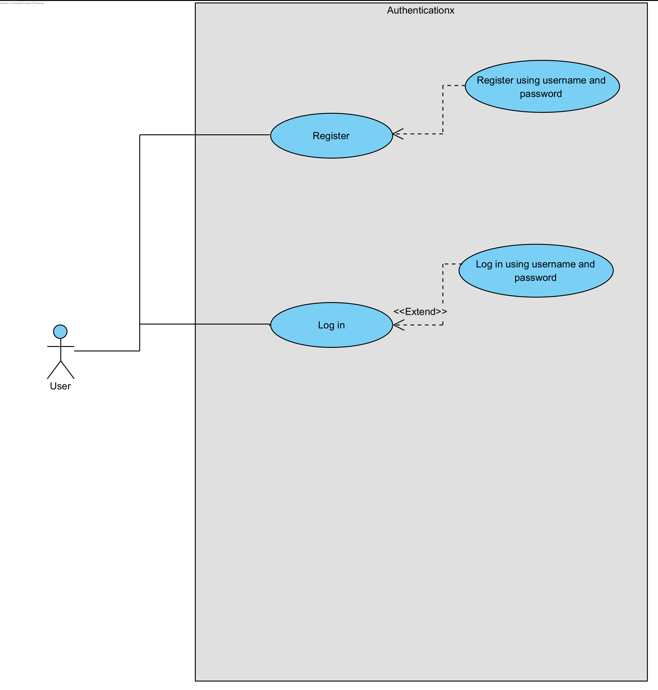
\includegraphics[width=13cm]{../../Images/UC2.2.1.png}
  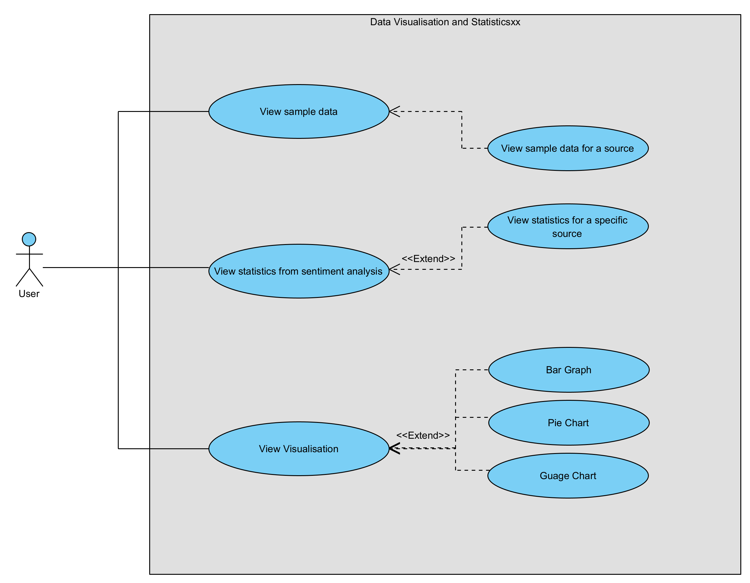
\includegraphics[width=13cm]{../../Images/UC2.2.2.png}
  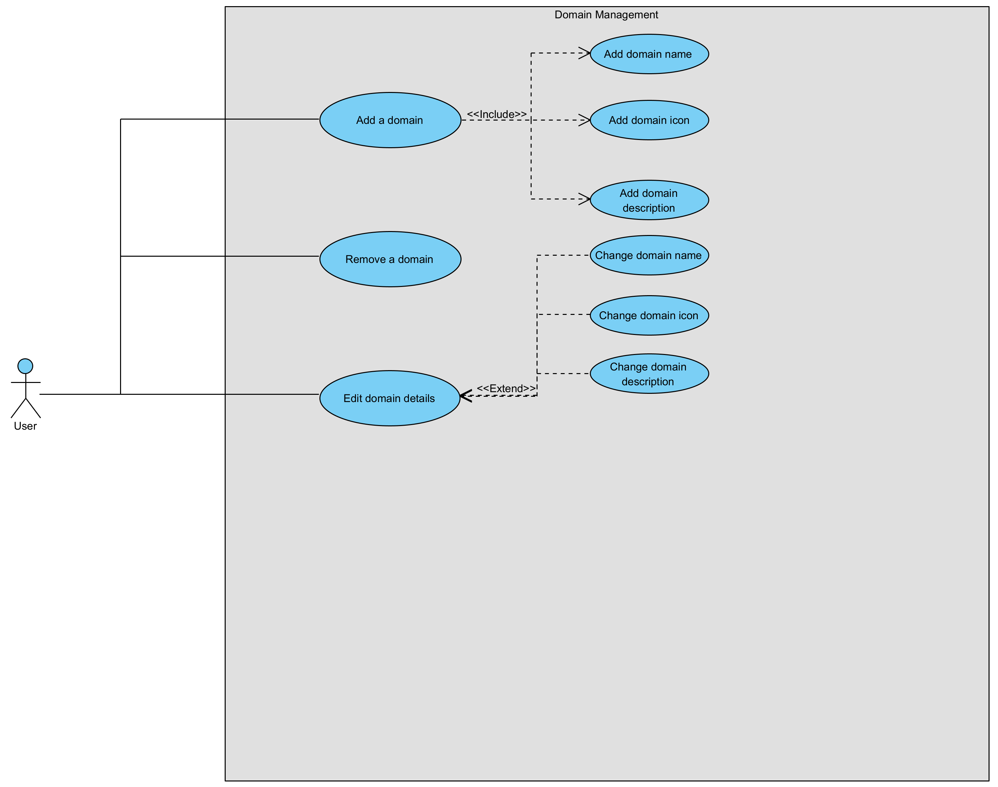
\includegraphics[width=13cm]{../../Images/UC2.2.3.png}
  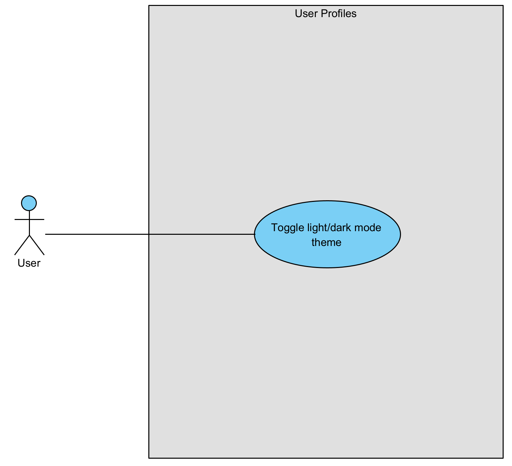
\includegraphics[width=13cm]{../../Images/UC2.2.4.png}
  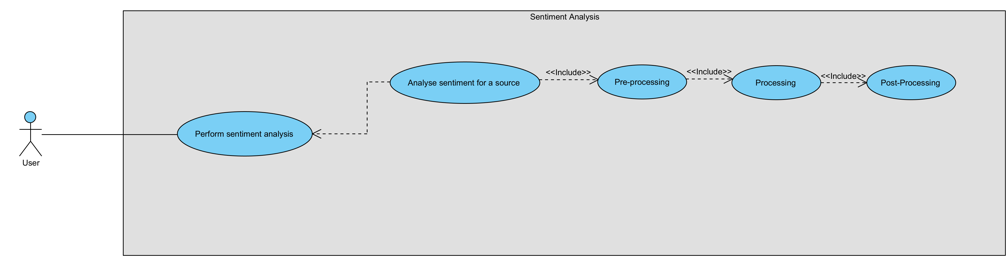
\includegraphics[width=13cm]{../../Images/UC2.2.5.png}
\end{center}

% \subsection{Eventual Use Case Diagrams}
% \begin{center}
%   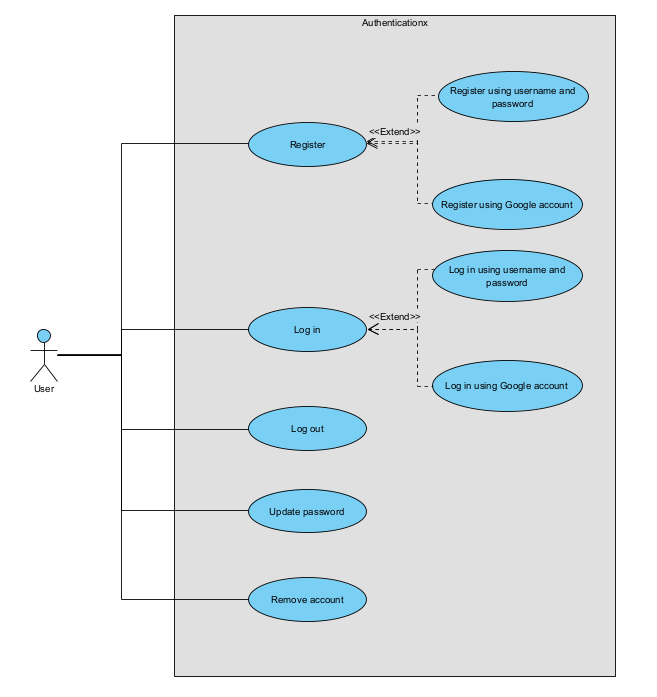
\includegraphics[width=13cm]{../../Images/UC 2.1.png}
%   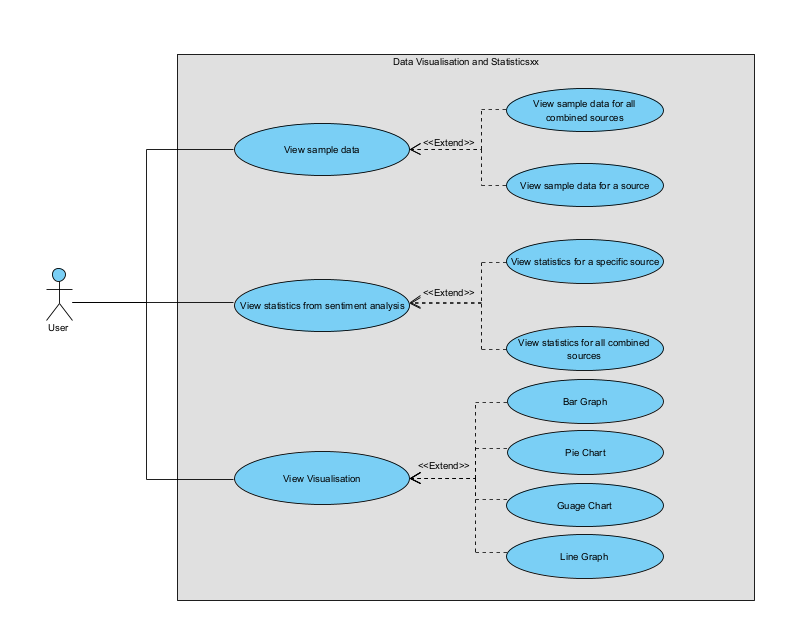
\includegraphics[width=13cm]{../../Images/UC 2.2.png}
%   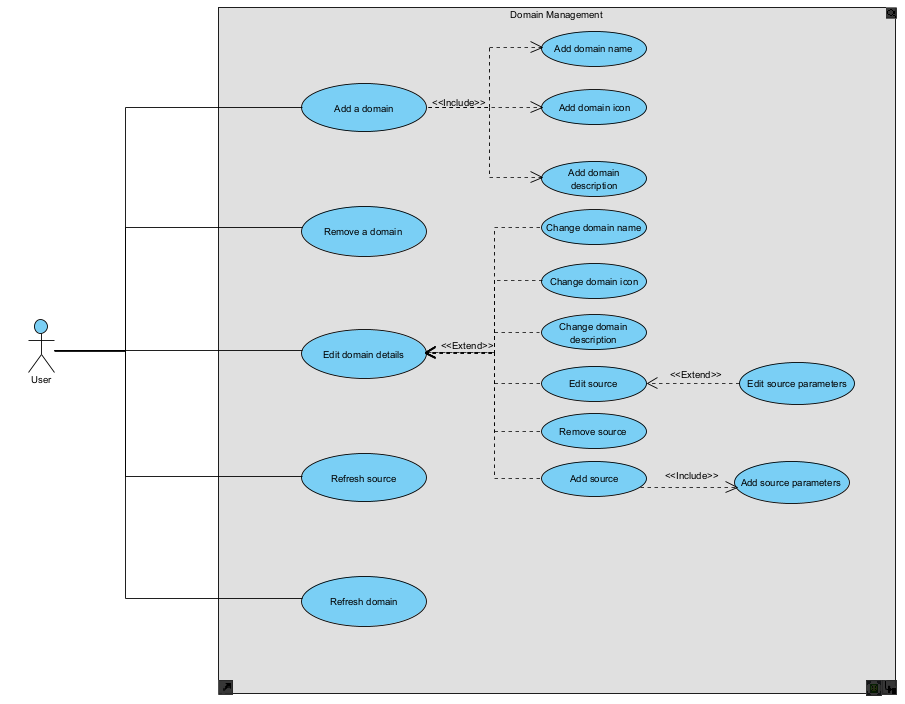
\includegraphics[width=13cm]{../../Images/UC 2.3.png}
%   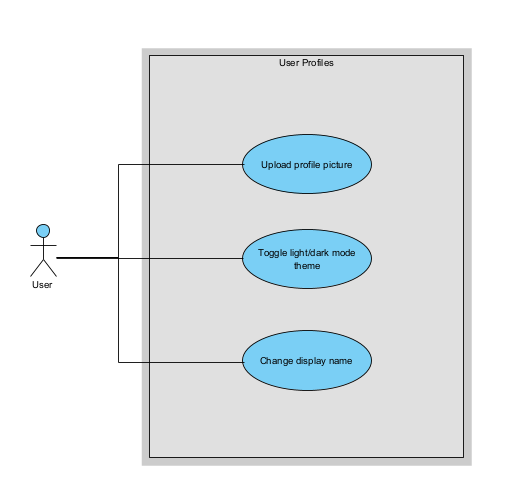
\includegraphics[width=13cm]{../../Images/UC 2.4.png}
%   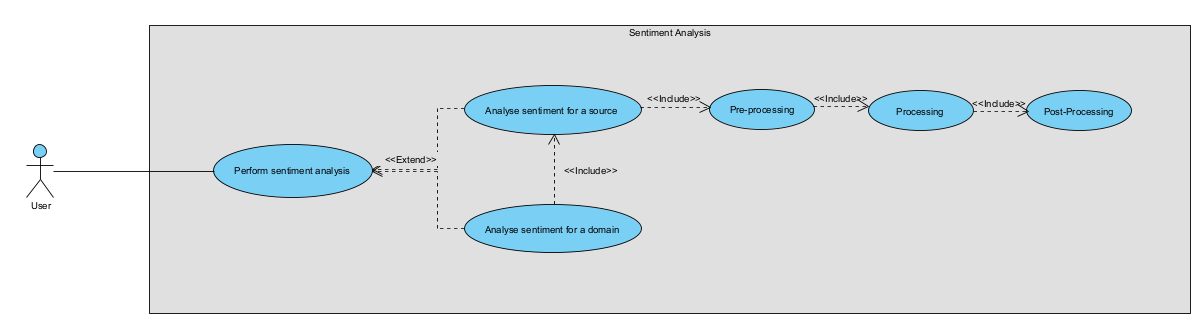
\includegraphics[width=13cm]{../../Images/UC 2.5.png}
% \end{center}






\newpage

\section{Service Contract}

\subsection{Provided Software}
As per the agreement between the client and development team, the software "Domain Pulse: A Sentiment Analysis Platform" shall be developed and deployed within the given time-frame. The system will allow users to register, create domains, add sources for the domains, and view aggregated and analyzed sentiment data from the sources.

\subsection{Technology Stack}
The system will be developed using Django as the backend web framework and Angular for the frontend UI. MongoDB, a NoSQL database, will be used for sentiment data storage, while PostgreSQL will be employed for user data storage. The system will be deployed and hosted on a client-provided virtual machine.

\subsection{Project Management}
The project will be managed using the Agile methodology, with weekly meetings between team members for effective communication and task coordination. GitHub Project Boards will be used to track tasks and progress. Biweekly meetings with the client will be conducted to provide progress reports and sprint reviews.

\subsection{Module Agreement}
The developed system will consist of external services and libraries within the codebase, comprising no more than 15\% of the total developed codebase. The team will ensure compliance with The University of Pretoria's Plagiarism and Code of Conduct policies, ensuring the originality and ownership of the produced code.

\subsection{Timeline}
The project will be completed within the provided time-frames of the COS 301 Capstone Project, and all required information and progress updates will be provided during the respective demos.

\subsection{Security}
Encryption will be implemented on all endpoints within the project to ensure secure data transmission between the server and the client. The virtual machine hosting the system will be secured and protected using measures such as firewalls. POST requests will be preferred over GET requests for enhanced data security.

\subsection{Law and User Privacy}
The software will comply with South African regulations, including laws such as the Protection of Personal Information Act (POPIA). User privacy and data will be protected and secured as required by the regulations.


\newpage

\section{Contract Design}

\subsection{Profile}

\subsubsection*{changeMode}
\textbf{Precondition:} \textit{mode: modeEnum} \\
\textbf{Postcondition:} Object of type 'Profile' corresponding to the user who made the method call containing the updated 'mode' is persistently stored and returned.

\subsubsection*{updateProfilePicture}
\textbf{Precondition:} \textit{pictureURL: string} \\
\textbf{Postcondition:} Object of type 'Profile' corresponding to the user who made the method call containing the updated 'profileIcon' is persistently stored and returned.

\subsection{User}
Authentication User Functions will be controlled by Django Authentication System

\subsubsection*{deleteProfile}
\textbf{Precondition:} \textit{userID: string} \\
\textbf{Postcondition:} A boolean is returned with true meaning 'success' and false meaning 'failure'

\subsubsection*{createProfile}
\textbf{Precondition:} \textit{profileIcon: string, mode: modeEnum} \\
\textbf{Postcondition:} Object of type 'Profile' containing the specified 'profileIcon', 'mode' and an empty array of strings (string[]) called domainID is persistently stored and returned.

\subsubsection*{getDomain}
\textbf{Precondition:} \textit{domainID: string} \\
\textbf{Postcondition:} The corresponding Domain Object is returned.

\subsection{Domain}

\subsubsection*{createDomain}
\textbf{Precondition:} \textit{name: string} \\
\textbf{Postcondition:} An Object of type Domain is returned and persistently stored containing the provided name, an empty description, icon and sources.

\subsubsection*{getDomains}
\textbf{Precondition:} \textit{userID: string} \\
\textbf{Postcondition:} An array of Domain objects is returned containing all domains and their relevant data.

\subsubsection*{editDomainDescription}
\textbf{Precondition:} \textit{description: string} \\
\textbf{Postcondition:} An Object of type Domain corresponding to the edited domain is returned and persistently stored, with the updated description value.

\subsubsection*{editDomainIcon}
\textbf{Precondition:} \textit{icon: string} \\
\textbf{Postcondition:} An Object of type Domain corresponding to the edited domain is returned and persistently stored with the updated icon value.

\subsubsection*{addSourceToDomain}
\textbf{Precondition:} \textit{newSource: Source} \\
\textbf{Postcondition:} An Object of type Domain corresponding to the edited domain is returned and persistently stored with the updated Sources array containing newSource.

\subsubsection*{deleteDomain}
\textbf{Precondition:} \textit{domainID: string} \\
\textbf{Postcondition:} A boolean is returned with true meaning 'success' and false meaning 'failure'.

\subsection{Source}

\subsubsection*{getSource}
\textbf{Precondition:} \textit{sourceID: string} \\
\textbf{PostCondition:} An Object of type Source with the passed in platform and query string value is returned.

\subsubsection*{createSource}
\textbf{Precondition:} \textit{platform: PlatformEnum, queryString: string} \\
\textbf{PostCondition:} An Object of type Source with the passed in platform and query string value is returned and persistently stored.

\subsubsection*{deleteSource}
\textbf{PreCondition:} \textit{sourceID: string} \\
\textbf{PostCondition:} A boolean is returned with true meaning 'success' and false meaning 'failure'.

\subsubsection*{editSource}
\textbf{Precondition:} \textit{queryString: string} \\
\textbf{PostCondition:} An Object of type Source corresponding to the edited source is returned and persistently stored with the queryString value.

\subsection{AnalysisEngine}

\subsubsection*{analyzeData}
\textbf{Precondition:} \textit{domain: Domain} \\
\textbf{Postcondition:} An array of SentimentMetrics objects corresponding to the stored sentiment records relating to the domain.

\subsubsection*{analyzeData}
\textbf{Precondition:} \textit{source: Source} \\
\textbf{Postcondition:} An array of SentimentMetrics objects corresponding to the stored sentiment records relating to the specific source of the domain.

\subsection{DataWarehouse}

\subsubsection*{getSentimentData}
\textbf{Precondition:} \textit{domainID: string} \\
\textbf{Postcondition:} An array of sentimentRecord objects is returned containing the records (comments, posts, etc.) pertaining to all sources of the domain provided.

\subsubsection*{fetchNewData}
\textbf{Precondition:} \textit{source: Source} \\
\textbf{Postcondition:} An array of sentimentRecord objects is persistently stored containing the records (comments, posts, etc.) pertaining to the specific source provided.

\subsubsection*{refreshSource}
\textbf{Precondition:} \textit{source: Source} \\
\textbf{PostCondition:} An array of sentimentRecord objects is returned and persistently stored containing the records (comments, posts, etc.) pertaining to the specific source provided.

\subsubsection*{getMetaData}
\textbf{Precondition:} \textit{source: Source} \\
\textbf{PostCondition:} An object is returned containing the number of pieces of data used in the source's data collection and the time taken for said data to be retrieved.

\subsubsection*{refreshAllSources}
\textbf{Precondition:} \textit{domain: Domain} \\
\textbf{Postcondition:} An array of sentimentRecords objects is returned and persistently stored containing the records (comments, posts, etc.) pertaining to all sources of the domain provided.

\subsection{Data Dashboard}

\subsubsection*{displayMetrics}
\textbf{Precondition:} \textit{domain: Domain} \\
\textbf{Postcondition:} The relevant data pertaining to the domain's sentiment metrics shall be displayed on the web page.

\subsubsection*{displayGraphs}
\textbf{Precondition:} \textit{domain: Domain} \\
\textbf{Postcondition:} The relevant graphs data pertaining to the domain's sentiment metrics shall be displayed on the web page.

\subsubsection*{displayMetrics}
\textbf{Precondition:} \textit{source: Source} \\
\textbf{Postcondition:} The relevant data pertaining to the domain's specific source sentiment metrics shall be displayed on the web page.

% \subsubsection*{displayGraphs}
% \textbf{Precondition:} \textit{source: Source} \\
% \textbf{Postcondition:} The relevant graphs pertaining to the domain's specific source sentiment metrics shall be displayed on the web page.


\newpage

\section{Database Design and Data Models}
The following is an outline of the structure of the data to be persisted and relationships between data entities. The system makes use of a combination of relational and document-based database technologies, hence the below diagram provides an overview.

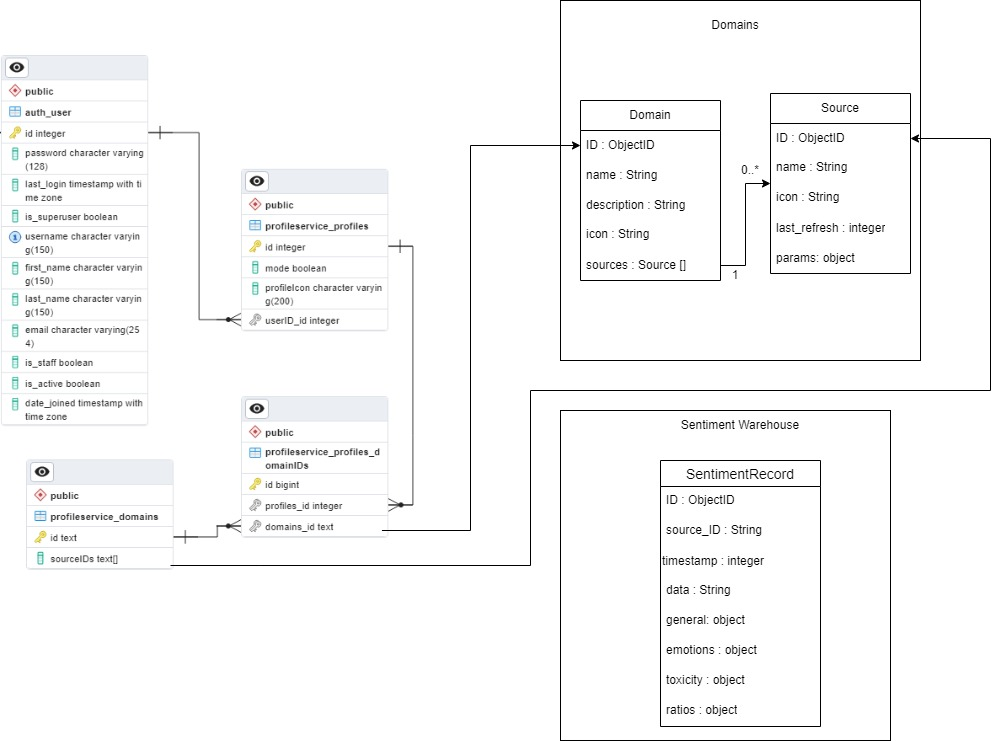
\includegraphics[width=13cm]{../../Images/DBDesign.jpg}\\\\

\newpage

\section{Class Diagram}

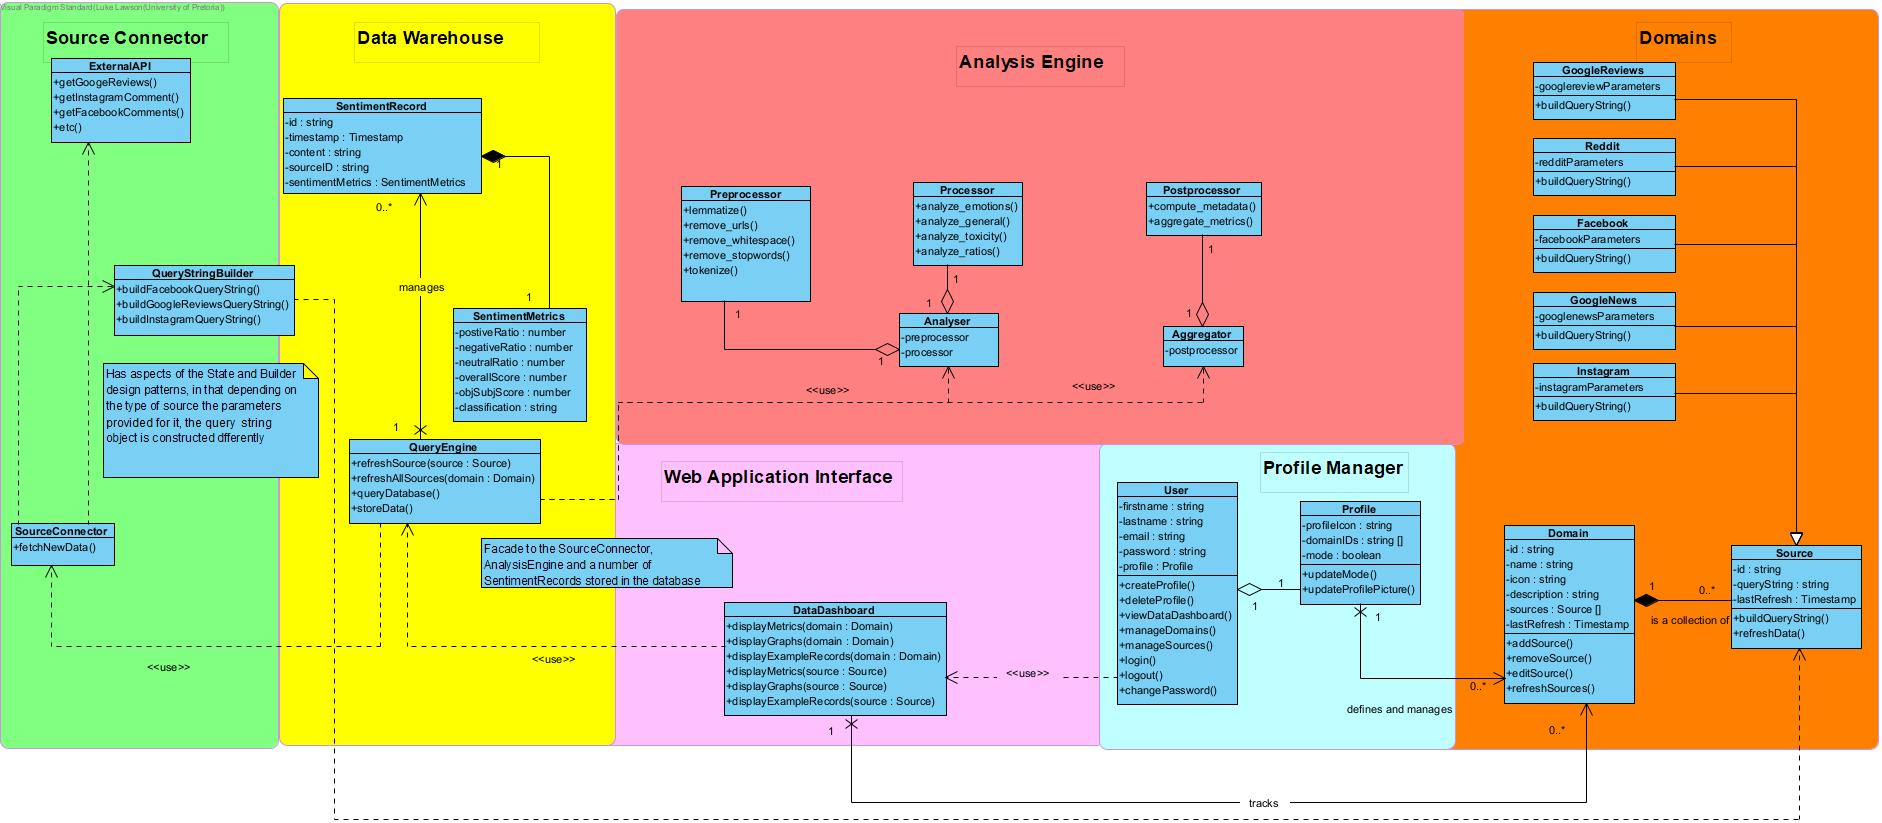
\includegraphics[width=13cm]{../../Images/classDiagram2.jpg}\\\\
\textbf{Design Patterns:} While the nature of the architecture does not lend itself to the Object-Oriented paradigm, two design patterns have been identified (and noted within the class diagram) - namely:\\\\
\textbf{Facade:} The \textit{QueryEngine} effectively acts as a \textit{Facade} to the \textit{SourceConnector}, the \textit{Analysis Engine}, and conceptually, to the database. This ensures that the \textit{QueryEngine} acts as a uniform interface to the frontend web-app (as well as the rest of the application in general) for the retrieval of data. That is, the rest of the system need not interact with the complicated underlying systems, but rather can communicate uniformly with the \textit{QueryEngine} (which abstracts out the complicated query logic involved with retrieving data from the database, from external APIs, or sending data for sentiment analysis in the \textit{AnalysisEngine}).\\\\
\textbf{Template Method:} Conceptually, the \textit{Template Method} design pattern is applied as follows: When a user defines a source, the source is categorized based on its type (e.g., Facebook, Reddit, etc). Each of these types of sources has different APIs with different parameters (and thus have different query strings). While the parent \textit{Source} class specifies the operation to build a query string, the individual, specific type of source defines exactly how that string may be built. i.e., The \textit{Source} is effectively a template for the construction of external API query strings, while the derivatives of the \textit{Source} (e.g., Reddit, Facebook, etc.) define how that template is "filled in" to construct the query string.



\newpage

\section{Constraints}

\textbf{Technical Constraints}
\begin{itemize}
  \item We are required to make use of a NoSQL document-based database in our application (upon specification from Southern Cross Solutions), however, upon request and their advice (given our architecture), it is acceptable to use a SQL database for services where we deem it necessary.
  \item All technology used for development must be free and open source (upon specification from Southern Cross Solutions).
\end{itemize}

\textbf{Performance Constraints}
\begin{itemize}
  \item Generally speaking, the following guidelines must be adhered to. Specific quantification of these requirements can be found in our statement of quality requirements and Testing Manual:
        \begin{itemize}
          \item The user must not wait for an inordinate amount of time for the data to be refreshed, including fetching new data from external APIs and performing analysis on that data.
          \item Viewing metrics for different sources and domains should feel seamless, with minimal waiting time involved in fetching the data.
          \item The web app needs to feel user-friendly, easy-to-use, and responsive.
        \end{itemize}
\end{itemize}

\textbf{Security Constraints}
\begin{itemize}
  \item User credentials must be stored with utmost care, ensuring that sensitive user information cannot be leaked and that another user may not gain unauthorized access to a user's account.
  \item The SSH keys provided to the team by Southern Cross Solutions cannot, under any circumstance, be leaked publicly and must only be sent across a secure platform.
\end{itemize}

\textbf{Regulatory Constraints}
\begin{itemize}
  \item Need to conform to the Terms of Service as specified by each external API we make use of.
  \item Need to ensure compliance with POPIA if we were to associate content with the person who posted it.
  \item Need to adhere to Southern Cross Solutions' company policy regarding keeping SSH keys to virtual machines secure.
\end{itemize}

\textbf{Cost Constraints}
\begin{itemize}
  \item Budget allocated for Project Day materials as well as an amount of no more than R300 towards making use of 3rd party web-scraping services.
\end{itemize}

\textbf{Time Constraints}
\begin{itemize}
  \item Need to have the final product delivered before the final demonstration and Project Day (approximately 6 months from start of development).
  \item Need to conform to milestone deadlines as set out by the requirements for demos 1 to 4.
\end{itemize}

\newpage

\section{Technology Requirements}

Below the technology requirements of the system are presented. All the mentioned technologies (with the exception of Azure and Outscraper) are free and open source. The justification of technology choices can be found in the Architectural Design Document.

\subsection{Development Environment}
For development, our team members shall be developing within VS Code in an Ubuntu Linux environment to ensure consistency within the produced code and testing of our software. Having all members using VS Code also allows for the use of software such as Live Share for collaborative development to improve efficiency within development.

\subsection{Version Control}
Git will be used for version control, using a clear and simple branching strategy that allows members to easily work on distinct components of our system while also allowing the reverting to previous versions as a 'fail-safe'. Meanwhile, GitHub will be used to host the Git repository.

\subsection{Programming Languages}
Within our team, all members have a high proficiency in coding in Python. Python is considered one of the best programming languages for Machine Learning and data analysis, which are aspects on which our system will heavily rely. Therefore, Python is our backend programming language of choice - along with the appropriate libraries for NLP, importing models, and other utility tasks. Frontend development will make use of standard languages: Typescript, CSS and HTML.

\subsection{Frameworks and Libraries}
We have decided to use Django as our web framework for the creation of our app due to its simplicity, efficiency, and secure data transmission capabilities. Within our Django project, we will be utilizing Python's proficiency in data analysis and machine learning by using a variety of powerful libraries for sentiment analysis and Natural Language Processing. For the front-end development, we will be using Angular due to its versatility and ability to create high-quality user interfaces.

\subsection{Database Systems}
For our database systems, we will be using MongoDB as a document-based NoSQL database for data collection of comments, posts, and other content related to user data. Additionally, PostgreSQL will be used as an SQL database for storing user profiles and authentication data for ease of access and querying.

\subsection{Testing and Quality Assurance Tools}
We will perform various forms of automated testing to ensure the quality of our software. For integration and E2E testing, Cypress will be used, and for unit testing, we will utilize the built-in Unittest library of Django Python, which is recommended for Django.

\subsection{Deployment and Infrastructure}
For deployment, our clients have provided a Linux-based virtual machine where we can deploy our software. We will use one virtual machine for the testing environment and another for the production environment (accessible with different domain names) to ensure a separation of concerns. Additionally, a domain may be acquired for ease of customer access to the software.

\subsection{Machine Learning and AI}
We will make use of a variety of open source, freely available, pre-trained sentiment analysis models. The BERT-style models are to be sourced from Hugging Face, while VADER is already available through the "vader" Python library.

\subsection{Collaboration and Communication Tools}
To ensure effective communication within our team, we have a private WhatsApp group for important announcements, a private Discord server for more specific announcements and discussions, and a private Signal group for sharing sensitive information such as secret keys, and a GitHub Project Board to track work progress. For communication with our clients, we have set up a Slack workspace for quick communication.

\subsection{Security and Encryption}
Our system is secured using technologies such as Django's authentication system, which encrypts user data. We prioritize the use of POST over GET for more secure data transmission. Our virtual machine is protected by extensive firewalls to prevent foreign attacks, and access is restricted to authorized members of our team using SSH and private login details.

\subsection{Continuous Integration and Deployment Tools}
We will utilize CI/CD technologies such as Codecov and GitHub Actions to ensure thorough testing and checking before deployment. GitHub Actions will automate the building, testing, and deployment processes, while Codecov will provide insights into test results and failures. We have been provided with separate production and testing environments to deploy and check the application's functionality.

\subsection{Hosting and Deployment}
Our clients, Southern Cross Solutions, have provisioned a virtual machine for us to host our application. Furthermore, we will be making use of Microsoft Azure cloud services for resource hosting and backup application hosting.

\subsection{Web Scraping}
In order to comply with the terms of service of the platforms from which Domain Pulse collects data, we will make use of Outscraper, a third party web scraping tool, to perform scraping on various review platforms such as Google Reviews and Tripadvisor. To retrieve data from Youtube, we will make use of the freely available Youtube Data v3 API, which allows us to retrieve comments on videos. 

\newpage



\end{document}
